\documentclass[tikz,border=0pt]{standalone}
\usepackage[T1]{fontenc}
\usepackage{newtxtext,newtxmath}
\usepackage{xcolor}
\definecolor{blue}{HTML}{326C9B}
\definecolor{gray}{HTML}{7F8993}
\definecolor{ink}{HTML}{203244}
\definecolor{grid}{HTML}{E5EAF0}
\definecolor{yellow}{HTML}{FFF19A}
\definecolor{orange}{HTML}{BD8547}
\definecolor{teal}{HTML}{488E85}
\begin{document}
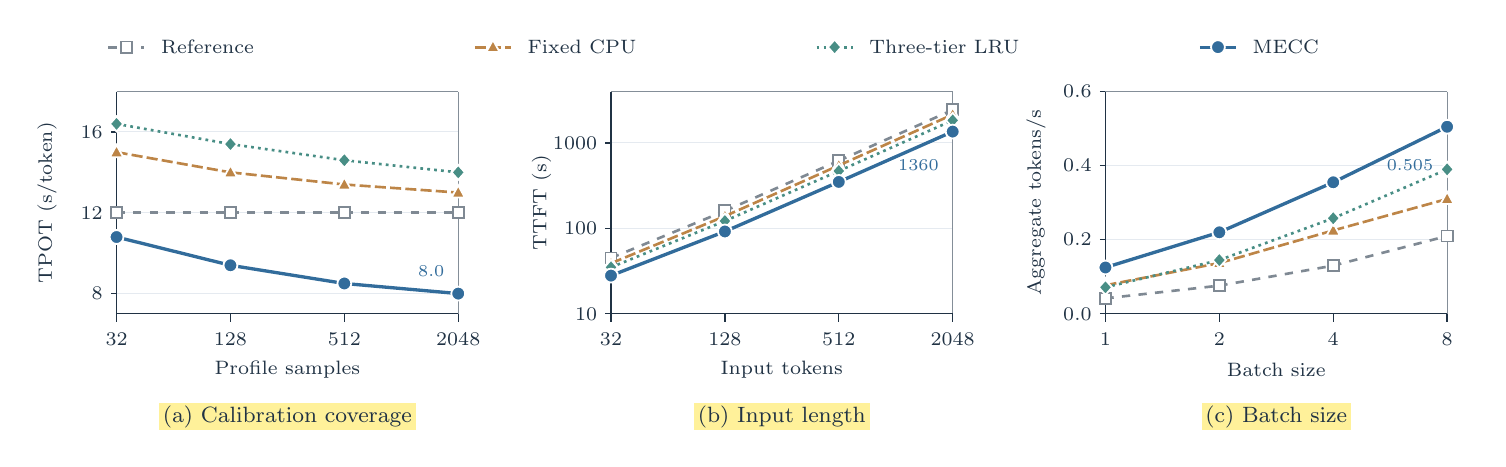
\begin{tikzpicture}[x=1bp,y=-1bp,every node/.style={inner sep=0pt,outer sep=0pt,text=ink,font=\fontsize{7.2}{8.2}\selectfont}]
\path[use as bounding box] (0,0) rectangle (522,148);
\draw[gray,line width=1.1bp,dashed] (29.000,7.000)--(42.000,7.000);
\filldraw[fill=white,draw=gray,line width=.65bp] (33.500,5.000) rectangle (37.500,9.000);
\node[anchor=west,text=ink,font=\fontsize{6.8}{7.8}\selectfont] at (48.000,7.000) {Reference};
\draw[orange,line width=1.1bp,dash pattern=on 4bp off 1.5bp] (161.000,7.000)--(174.000,7.000);
\filldraw[fill=orange,draw=white,line width=.65bp] (167.500,4.400)--(165.100,8.800)--(169.900,8.800)--cycle;
\node[anchor=west,text=ink,font=\fontsize{6.8}{7.8}\selectfont] at (180.000,7.000) {Fixed CPU};
\draw[teal,line width=1.1bp,dash pattern=on 1bp off 1.5bp] (284.000,7.000)--(297.000,7.000);
\filldraw[fill=teal,draw=white,line width=.65bp] (290.500,4.300)--(288.100,7.000)--(290.500,9.700)--(292.900,7.000)--cycle;
\node[anchor=west,text=ink,font=\fontsize{6.8}{7.8}\selectfont] at (303.000,7.000) {Three-tier LRU};
\draw[blue,line width=1.1bp] (422.000,7.000)--(435.000,7.000);
\filldraw[fill=blue,draw=white,line width=.65bp] (428.500,7.000) circle[radius=2.5bp];
\node[anchor=west,text=ink,font=\fontsize{6.8}{7.8}\selectfont] at (441.000,7.000) {MECC};
\draw[grid,line width=0.35bp] (32.000,95.727)--(155.000,95.727);
\draw[ink,line width=0.45bp] (30.000,95.727)--(32.000,95.727);
\node[anchor=east,text=ink,font=\fontsize{6.7}{7.7}\selectfont] at (27.000,95.727) {8};
\draw[grid,line width=0.35bp] (32.000,66.636)--(155.000,66.636);
\draw[ink,line width=0.45bp] (30.000,66.636)--(32.000,66.636);
\node[anchor=east,text=ink,font=\fontsize{6.7}{7.7}\selectfont] at (27.000,66.636) {12};
\draw[grid,line width=0.35bp] (32.000,37.545)--(155.000,37.545);
\draw[ink,line width=0.45bp] (30.000,37.545)--(32.000,37.545);
\node[anchor=east,text=ink,font=\fontsize{6.7}{7.7}\selectfont] at (27.000,37.545) {16};
\draw[ink!55,line width=0.4bp] (32.000,23.000)--(155.000,23.000);
\draw[ink!55,line width=0.4bp] (155.000,23.000)--(155.000,103.000);
\draw[ink,line width=0.5bp] (32.000,23.000)--(32.000,103.000);
\draw[ink,line width=0.5bp] (32.000,103.000)--(155.000,103.000);
\draw[gray,line width=0.95bp,dashed] (32.000,66.636)--(73.000,66.636);
\draw[gray,line width=0.95bp,dashed] (73.000,66.636)--(114.000,66.636);
\draw[gray,line width=0.95bp,dashed] (114.000,66.636)--(155.000,66.636);
\filldraw[fill=white,draw=gray,line width=.65bp] (30.000,64.636) rectangle (34.000,68.636);
\filldraw[fill=white,draw=gray,line width=.65bp] (71.000,64.636) rectangle (75.000,68.636);
\filldraw[fill=white,draw=gray,line width=.65bp] (112.000,64.636) rectangle (116.000,68.636);
\filldraw[fill=white,draw=gray,line width=.65bp] (153.000,64.636) rectangle (157.000,68.636);
\draw[orange,line width=0.95bp,dash pattern=on 4bp off 1.5bp] (32.000,44.818)--(73.000,52.091);
\draw[orange,line width=0.95bp,dash pattern=on 4bp off 1.5bp] (73.000,52.091)--(114.000,56.455);
\draw[orange,line width=0.95bp,dash pattern=on 4bp off 1.5bp] (114.000,56.455)--(155.000,59.364);
\filldraw[fill=orange,draw=white,line width=.65bp] (32.000,42.218)--(29.600,46.618)--(34.400,46.618)--cycle;
\filldraw[fill=orange,draw=white,line width=.65bp] (73.000,49.491)--(70.600,53.891)--(75.400,53.891)--cycle;
\filldraw[fill=orange,draw=white,line width=.65bp] (114.000,53.855)--(111.600,58.255)--(116.400,58.255)--cycle;
\filldraw[fill=orange,draw=white,line width=.65bp] (155.000,56.764)--(152.600,61.164)--(157.400,61.164)--cycle;
\draw[teal,line width=0.95bp,dash pattern=on 1bp off 1.5bp] (32.000,34.636)--(73.000,41.909);
\draw[teal,line width=0.95bp,dash pattern=on 1bp off 1.5bp] (73.000,41.909)--(114.000,47.727);
\draw[teal,line width=0.95bp,dash pattern=on 1bp off 1.5bp] (114.000,47.727)--(155.000,52.091);
\filldraw[fill=teal,draw=white,line width=.65bp] (32.000,31.936)--(29.600,34.636)--(32.000,37.336)--(34.400,34.636)--cycle;
\filldraw[fill=teal,draw=white,line width=.65bp] (73.000,39.209)--(70.600,41.909)--(73.000,44.609)--(75.400,41.909)--cycle;
\filldraw[fill=teal,draw=white,line width=.65bp] (114.000,45.027)--(111.600,47.727)--(114.000,50.427)--(116.400,47.727)--cycle;
\filldraw[fill=teal,draw=white,line width=.65bp] (155.000,49.391)--(152.600,52.091)--(155.000,54.791)--(157.400,52.091)--cycle;
\draw[blue,line width=1.2bp] (32.000,75.364)--(73.000,85.545);
\draw[blue,line width=1.2bp] (73.000,85.545)--(114.000,92.091);
\draw[blue,line width=1.2bp] (114.000,92.091)--(155.000,95.727);
\filldraw[fill=blue,draw=white,line width=.65bp] (32.000,75.364) circle[radius=2.5bp];
\filldraw[fill=blue,draw=white,line width=.65bp] (73.000,85.545) circle[radius=2.5bp];
\filldraw[fill=blue,draw=white,line width=.65bp] (114.000,92.091) circle[radius=2.5bp];
\filldraw[fill=blue,draw=white,line width=.65bp] (155.000,95.727) circle[radius=2.5bp];
\draw[ink,line width=0.45bp] (32.000,103.000)--(32.000,106.000);
\node[anchor=center,text=ink,font=\fontsize{6.7}{7.7}\selectfont] at (32.000,112.000) {32};
\draw[ink,line width=0.45bp] (73.000,103.000)--(73.000,106.000);
\node[anchor=center,text=ink,font=\fontsize{6.7}{7.7}\selectfont] at (73.000,112.000) {128};
\draw[ink,line width=0.45bp] (114.000,103.000)--(114.000,106.000);
\node[anchor=center,text=ink,font=\fontsize{6.7}{7.7}\selectfont] at (114.000,112.000) {512};
\draw[ink,line width=0.45bp] (155.000,103.000)--(155.000,106.000);
\node[anchor=center,text=ink,font=\fontsize{6.7}{7.7}\selectfont] at (155.000,112.000) {2048};
\node[anchor=center,text=ink,font=\fontsize{7.2}{8.2}\selectfont,rotate=90] at (7.000,63.000) {TPOT (s/token)};
\node[anchor=center,text=ink,font=\fontsize{7.2}{8.2}\selectfont] at (93.500,123.000) {Profile samples};
\node[anchor=center,text=ink,font=\fontsize{7.8}{8.8}\selectfont,fill=yellow,inner xsep=1.4bp,inner ysep=1.0bp] at (93.500,140.000) {(a) Calibration coverage};
\node[anchor=east,text=blue,font=\fontsize{6.5}{7.5}\selectfont] at (150.000,87.727) {8.0};
\draw[grid,line width=0.35bp] (210.000,103.000)--(333.000,103.000);
\draw[ink,line width=0.45bp] (208.000,103.000)--(210.000,103.000);
\node[anchor=east,text=ink,font=\fontsize{6.7}{7.7}\selectfont] at (205.000,103.000) {10};
\draw[grid,line width=0.35bp] (210.000,72.255)--(333.000,72.255);
\draw[ink,line width=0.45bp] (208.000,72.255)--(210.000,72.255);
\node[anchor=east,text=ink,font=\fontsize{6.7}{7.7}\selectfont] at (205.000,72.255) {100};
\draw[grid,line width=0.35bp] (210.000,41.510)--(333.000,41.510);
\draw[ink,line width=0.45bp] (208.000,41.510)--(210.000,41.510);
\node[anchor=east,text=ink,font=\fontsize{6.7}{7.7}\selectfont] at (205.000,41.510) {1000};
\draw[ink!55,line width=0.4bp] (210.000,23.000)--(333.000,23.000);
\draw[ink!55,line width=0.4bp] (333.000,23.000)--(333.000,103.000);
\draw[ink,line width=0.5bp] (210.000,23.000)--(210.000,103.000);
\draw[ink,line width=0.5bp] (210.000,103.000)--(333.000,103.000);
\draw[gray,line width=0.95bp,dashed] (210.000,82.917)--(251.000,65.979);
\draw[gray,line width=0.95bp,dashed] (251.000,65.979)--(292.000,47.893);
\draw[gray,line width=0.95bp,dashed] (292.000,47.893)--(333.000,29.600);
\filldraw[fill=white,draw=gray,line width=.65bp] (208.000,80.917) rectangle (212.000,84.917);
\filldraw[fill=white,draw=gray,line width=.65bp] (249.000,63.979) rectangle (253.000,67.979);
\filldraw[fill=white,draw=gray,line width=.65bp] (290.000,45.893) rectangle (294.000,49.893);
\filldraw[fill=white,draw=gray,line width=.65bp] (331.000,27.600) rectangle (335.000,31.600);
\draw[orange,line width=0.95bp,dash pattern=on 4bp off 1.5bp] (210.000,84.828)--(251.000,67.858);
\draw[orange,line width=0.95bp,dash pattern=on 4bp off 1.5bp] (251.000,67.858)--(292.000,49.615);
\draw[orange,line width=0.95bp,dash pattern=on 4bp off 1.5bp] (292.000,49.615)--(333.000,31.289);
\filldraw[fill=orange,draw=white,line width=.65bp] (210.000,82.228)--(207.600,86.628)--(212.400,86.628)--cycle;
\filldraw[fill=orange,draw=white,line width=.65bp] (251.000,65.258)--(248.600,69.658)--(253.400,69.658)--cycle;
\filldraw[fill=orange,draw=white,line width=.65bp] (292.000,47.015)--(289.600,51.415)--(294.400,51.415)--cycle;
\filldraw[fill=orange,draw=white,line width=.65bp] (333.000,28.689)--(330.600,33.089)--(335.400,33.089)--cycle;
\draw[teal,line width=0.95bp,dash pattern=on 1bp off 1.5bp] (210.000,86.273)--(251.000,69.600);
\draw[teal,line width=0.95bp,dash pattern=on 1bp off 1.5bp] (251.000,69.600)--(292.000,51.592);
\draw[teal,line width=0.95bp,dash pattern=on 1bp off 1.5bp] (292.000,51.592)--(333.000,33.368);
\filldraw[fill=teal,draw=white,line width=.65bp] (210.000,83.573)--(207.600,86.273)--(210.000,88.973)--(212.400,86.273)--cycle;
\filldraw[fill=teal,draw=white,line width=.65bp] (251.000,66.900)--(248.600,69.600)--(251.000,72.300)--(253.400,69.600)--cycle;
\filldraw[fill=teal,draw=white,line width=.65bp] (292.000,48.892)--(289.600,51.592)--(292.000,54.292)--(294.400,51.592)--cycle;
\filldraw[fill=teal,draw=white,line width=.65bp] (333.000,30.668)--(330.600,33.368)--(333.000,36.068)--(335.400,33.368)--cycle;
\draw[blue,line width=1.2bp] (210.000,89.252)--(251.000,73.368);
\draw[blue,line width=1.2bp] (251.000,73.368)--(292.000,55.528);
\draw[blue,line width=1.2bp] (292.000,55.528)--(333.000,37.405);
\filldraw[fill=blue,draw=white,line width=.65bp] (210.000,89.252) circle[radius=2.5bp];
\filldraw[fill=blue,draw=white,line width=.65bp] (251.000,73.368) circle[radius=2.5bp];
\filldraw[fill=blue,draw=white,line width=.65bp] (292.000,55.528) circle[radius=2.5bp];
\filldraw[fill=blue,draw=white,line width=.65bp] (333.000,37.405) circle[radius=2.5bp];
\draw[ink,line width=0.45bp] (210.000,103.000)--(210.000,106.000);
\node[anchor=center,text=ink,font=\fontsize{6.7}{7.7}\selectfont] at (210.000,112.000) {32};
\draw[ink,line width=0.45bp] (251.000,103.000)--(251.000,106.000);
\node[anchor=center,text=ink,font=\fontsize{6.7}{7.7}\selectfont] at (251.000,112.000) {128};
\draw[ink,line width=0.45bp] (292.000,103.000)--(292.000,106.000);
\node[anchor=center,text=ink,font=\fontsize{6.7}{7.7}\selectfont] at (292.000,112.000) {512};
\draw[ink,line width=0.45bp] (333.000,103.000)--(333.000,106.000);
\node[anchor=center,text=ink,font=\fontsize{6.7}{7.7}\selectfont] at (333.000,112.000) {2048};
\node[anchor=center,text=ink,font=\fontsize{7.2}{8.2}\selectfont,rotate=90] at (185.000,63.000) {TTFT (s)};
\node[anchor=center,text=ink,font=\fontsize{7.2}{8.2}\selectfont] at (271.500,123.000) {Input tokens};
\node[anchor=center,text=ink,font=\fontsize{7.8}{8.8}\selectfont,fill=yellow,inner xsep=1.4bp,inner ysep=1.0bp] at (271.500,140.000) {(b) Input length};
\node[anchor=east,text=blue,font=\fontsize{6.5}{7.5}\selectfont] at (328.000,49.405) {1360};
\draw[grid,line width=0.35bp] (388.000,103.000)--(511.000,103.000);
\draw[ink,line width=0.45bp] (386.000,103.000)--(388.000,103.000);
\node[anchor=east,text=ink,font=\fontsize{6.7}{7.7}\selectfont] at (383.000,103.000) {0.0};
\draw[grid,line width=0.35bp] (388.000,76.333)--(511.000,76.333);
\draw[ink,line width=0.45bp] (386.000,76.333)--(388.000,76.333);
\node[anchor=east,text=ink,font=\fontsize{6.7}{7.7}\selectfont] at (383.000,76.333) {0.2};
\draw[grid,line width=0.35bp] (388.000,49.667)--(511.000,49.667);
\draw[ink,line width=0.45bp] (386.000,49.667)--(388.000,49.667);
\node[anchor=east,text=ink,font=\fontsize{6.7}{7.7}\selectfont] at (383.000,49.667) {0.4};
\draw[grid,line width=0.35bp] (388.000,23.000)--(511.000,23.000);
\draw[ink,line width=0.45bp] (386.000,23.000)--(388.000,23.000);
\node[anchor=east,text=ink,font=\fontsize{6.7}{7.7}\selectfont] at (383.000,23.000) {0.6};
\draw[ink!55,line width=0.4bp] (388.000,23.000)--(511.000,23.000);
\draw[ink!55,line width=0.4bp] (511.000,23.000)--(511.000,103.000);
\draw[ink,line width=0.5bp] (388.000,23.000)--(388.000,103.000);
\draw[ink,line width=0.5bp] (388.000,103.000)--(511.000,103.000);
\draw[gray,line width=0.95bp,dashed] (388.000,97.444)--(429.000,92.867);
\draw[gray,line width=0.95bp,dashed] (429.000,92.867)--(470.000,85.667);
\draw[gray,line width=0.95bp,dashed] (470.000,85.667)--(511.000,75.000);
\filldraw[fill=white,draw=gray,line width=.65bp] (386.000,95.444) rectangle (390.000,99.444);
\filldraw[fill=white,draw=gray,line width=.65bp] (427.000,90.867) rectangle (431.000,94.867);
\filldraw[fill=white,draw=gray,line width=.65bp] (468.000,83.667) rectangle (472.000,87.667);
\filldraw[fill=white,draw=gray,line width=.65bp] (509.000,73.000) rectangle (513.000,77.000);
\draw[orange,line width=0.95bp,dash pattern=on 4bp off 1.5bp] (388.000,92.744)--(429.000,84.733);
\draw[orange,line width=0.95bp,dash pattern=on 4bp off 1.5bp] (429.000,84.733)--(470.000,73.000);
\draw[orange,line width=0.95bp,dash pattern=on 4bp off 1.5bp] (470.000,73.000)--(511.000,61.667);
\filldraw[fill=orange,draw=white,line width=.65bp] (388.000,90.144)--(385.600,94.544)--(390.400,94.544)--cycle;
\filldraw[fill=orange,draw=white,line width=.65bp] (429.000,82.133)--(426.600,86.533)--(431.400,86.533)--cycle;
\filldraw[fill=orange,draw=white,line width=.65bp] (470.000,70.400)--(467.600,74.800)--(472.400,74.800)--cycle;
\filldraw[fill=orange,draw=white,line width=.65bp] (511.000,59.067)--(508.600,63.467)--(513.400,63.467)--cycle;
\draw[teal,line width=0.95bp,dash pattern=on 1bp off 1.5bp] (388.000,93.476)--(429.000,83.667);
\draw[teal,line width=0.95bp,dash pattern=on 1bp off 1.5bp] (429.000,83.667)--(470.000,68.600);
\draw[teal,line width=0.95bp,dash pattern=on 1bp off 1.5bp] (470.000,68.600)--(511.000,51.000);
\filldraw[fill=teal,draw=white,line width=.65bp] (388.000,90.776)--(385.600,93.476)--(388.000,96.176)--(390.400,93.476)--cycle;
\filldraw[fill=teal,draw=white,line width=.65bp] (429.000,80.967)--(426.600,83.667)--(429.000,86.367)--(431.400,83.667)--cycle;
\filldraw[fill=teal,draw=white,line width=.65bp] (470.000,65.900)--(467.600,68.600)--(470.000,71.300)--(472.400,68.600)--cycle;
\filldraw[fill=teal,draw=white,line width=.65bp] (511.000,48.300)--(508.600,51.000)--(511.000,53.700)--(513.400,51.000)--cycle;
\draw[blue,line width=1.2bp] (388.000,86.333)--(429.000,73.667);
\draw[blue,line width=1.2bp] (429.000,73.667)--(470.000,55.667);
\draw[blue,line width=1.2bp] (470.000,55.667)--(511.000,35.667);
\filldraw[fill=blue,draw=white,line width=.65bp] (388.000,86.333) circle[radius=2.5bp];
\filldraw[fill=blue,draw=white,line width=.65bp] (429.000,73.667) circle[radius=2.5bp];
\filldraw[fill=blue,draw=white,line width=.65bp] (470.000,55.667) circle[radius=2.5bp];
\filldraw[fill=blue,draw=white,line width=.65bp] (511.000,35.667) circle[radius=2.5bp];
\draw[ink,line width=0.45bp] (388.000,103.000)--(388.000,106.000);
\node[anchor=center,text=ink,font=\fontsize{6.7}{7.7}\selectfont] at (388.000,112.000) {1};
\draw[ink,line width=0.45bp] (429.000,103.000)--(429.000,106.000);
\node[anchor=center,text=ink,font=\fontsize{6.7}{7.7}\selectfont] at (429.000,112.000) {2};
\draw[ink,line width=0.45bp] (470.000,103.000)--(470.000,106.000);
\node[anchor=center,text=ink,font=\fontsize{6.7}{7.7}\selectfont] at (470.000,112.000) {4};
\draw[ink,line width=0.45bp] (511.000,103.000)--(511.000,106.000);
\node[anchor=center,text=ink,font=\fontsize{6.7}{7.7}\selectfont] at (511.000,112.000) {8};
\node[anchor=center,text=ink,font=\fontsize{7.2}{8.2}\selectfont,rotate=90] at (363.000,63.000) {Aggregate tokens/s};
\node[anchor=center,text=ink,font=\fontsize{7.2}{8.2}\selectfont] at (449.500,123.000) {Batch size};
\node[anchor=center,text=ink,font=\fontsize{7.8}{8.8}\selectfont,fill=yellow,inner xsep=1.4bp,inner ysep=1.0bp] at (449.500,140.000) {(c) Batch size};
\node[anchor=east,text=blue,font=\fontsize{6.5}{7.5}\selectfont] at (506.000,49.667) {0.505};
\end{tikzpicture}
\end{document}
